This chapter presents the evaluated policies on different RL problems. 
First, the setup and the used drone model is shortly defined by the different static and dynamic parameters. 
The main part of this chapter are the different results of a variety of policies on fixed goal modes, random goal modes and modes using wind disruption. 
The policies may differ in terms of actions, type of training, control frequency and RL algorithm, but all aim at different partial aspects of controlling a drone via RL.

\section{Drone Model \& Setup}
The used drone model $DroneModel.HB$ is part of the Gym-Pybullets-Drones package and is defined by its parameters (\cref{tab:drone}): 
the arm length, the thrust to weight ratio, the maximum speed, the mass and two constants $k_f, k_m$, which directly influence the forces and torques.
The mass of $0.5kg$ should help to counteract wind as well as the huge maximum speed of $50 \frac{km}{h}$.\\
The agents were learned on a pc equipped with a \emph{NVIDIA GeForce RTX 4090} in order to reduce training time. 
Still, the training time for each policy was inside a span of $0.5h$ to $3d$, mostly depending on the amount of training steps and the used RL algorithm.

\begin{table}
	\centering
	\caption{Parameters of used drone model}\label{tab:drone}
	\begin{tabular}{|c|c|c|c|c|c|}
		\hline
		Arm & $k_f$& $k_m$ & $t2w$ & $|\dot{v}|$ & $m$ \\
		\hline
		$0.175m$ & $6.11e-8$ & $1.5e-9$ & $2$ & $50 \frac{km}{h}$ & $0.5 kg$\\
		\hline
	\end{tabular}
\end{table}


\section{Results}
The results are structures into the results of the fixed goal modes, the random goal modes and in general wind disruption. 
This section aims at examining different algorithms and methods for control of flying drones in goal environments 
on a metric which combines classic RL performance parameters like the reward $r_e$, but also classic control theory parameters like 
success rate, time rate $\beth$, distances during the simulation, the overshoot and a settling rate. 
In addition, it uses different kinds of optimality and expected optimality, 
which relates certain metric parameters to its theoretical optimal value.

\subsection{Fixed Goal Modes}
On fixed goal modes the policies are introduced at first and their training is compared. 
Then 4D action and 1D action models are compared, mostly regarding the resulting rpm logs. 
The main part is an overall comparison of the models and a comparison for different episode lengths in order 
to explain which algorithm seems to be better at generalizing the fixed goal RL problem. 
At last, different policies are evaluated that have been trained with different control frequencies $\frac{f_s}{\aleph}$ on environments with different control frequencies. 
This aims at comparing the policies on their robustness to control frequencies.
%In total, this subsection aims at comparing the PPO and SAC algorithm and examine whether any of them produces a policy good enough for real flight. 

\subsubsection{Policies}
This section uses a total of six different policies (\cref{tab:pi1}).
\emph{PPO1D\_1.zip} and \\ \emph{SAC1D\_1.zip} were both trained on a mode 1 environment with $5e6$ steps and a 1 dimensional action, 
but only differ in the used algorithm.
 \emph{PPO4D\_1.zip} was trained with a total amount of $3e7$ steps. Also, the dimensionality of the action increases to four.
 \emph{SAC4D\_1.zip} and \emph{SAC4D48\_1.zip} only differ in the used control frequency, but operate with the same action and were both learned with the SAC algorithm.
 \emph{$\pi_{opt}$} is the theoretical construct of the optimal policy for this RL problems based on \cref{sec:oprew}. 
 It always takes the optimal action therefore defines the best possible reward $r_opt$ that depends on mode and control frequency and the optimal time rate $\beth_{opt}$.
 In mode 0 the action is always (0, 0, 0, 0). 
 Due to processing the hover\_rpm is applied, and the drone stays in the goal. 
 In mode 1 it takes the action (1, 1, 1, 1) as long as possible and then brakes into the goal. 
 There it also applies (0, 0, 0, 0). The optimal reward and time rate can then be expressed as \cref{eq:optrew} and \cref{eq:optt}.
 
 \begin{align}
 	r_{opt} &=
 	\left\{
 	\begin{array}{ll}
 		0 & \mbox{if } mode = 0\\
 		-4.874 &\mbox{if } mode = 1 \land \frac{f_s}{\aleph} = 48Hz\\
 		-2.39 &\mbox{if } mode = 1 \land \frac{f_s}{\aleph} = 24Hz\\
 	\end{array}
 	\right. \label{eq:optrew}\\
 	\beth_{opt} &= 
 	\left\{
 	\begin{array}{ll}
 		1 & \mbox{if } mode = 0\\
 		0.83750 &\mbox{if } mode = 1 \\
 	\end{array}
 	\right. \label{eq:optt}
 \end{align}


\begin{longtable}{|c|c|c|c|c|c|}
	\caption{Overview of the evaluated Policies on fixed goal modes}\label{tab:pi1}\\
	
	\hline
	Name & Algorithm & ActionType & $\frac{f_s}{\aleph}$ & $t_{total}$ & Mode\\
	\hline
	%\toprule
	\endfirsthead
	\caption[]{Overview of the evaluated Policies on fixed goal modes}
	\endhead
%	PPO4D\_0.zip & PPO & $rpm$ & $48Hz$ & $5e6$ & 0\\
%	\hline
%	SAC4D\_0.zip & SAC & $rpm$ & $48Hz$ & $5e6$ & 0\\
%	\hline
	PPO1D\_1.zip & PPO & $one\_d\_rpm$ & $48 Hz$ & $5e6$ & 1\\
	\hline
	SAC1D\_1.zip & SAC & $one\_d\_rpm$ & $48 Hz$ & $5e6$ & 1\\
	\hline
	PPO4D\_1.zip & PPO & $rpm$ & $48Hz$ & $3e7$ & 1\\
	\hline
	SAC4D24\_1.zip & SAC & $rpm$ & $24Hz$ & $3e7$ & 1\\
	\hline
	SAC4D48\_1.zip & SAC & $rpm$ & $24Hz$ & $3e7$ & 1\\
	\hline
	$\pi_{opt}$ & & & & & \\
	\hline
\end{longtable}

\newpage

\subsubsection{Training Comparison}
%1D policies 
%4D policies

\newpage

\subsubsection{Action Comparison}
% log of 1D rpms
% log of 4D rpms

\newpage

\subsubsection{Overall Comparison}

\begin{longtable}{|c|c|c|c|c|c|}
	\caption{Evaluation of the Policies with mode 1}\label{tab:eval0}\\
	
	\hline
	& PPO1D & SAC1D & PPO4D & SAC4D24 & SAC4D48 \\
	\hline
	%\toprule
	\endfirsthead
	\caption[]{Evaluation of the Policies with mode 1}
	\endhead
	\hline
	Reward $r_e$ & & & $-6.036$ & $-7.325$ & $-7.717$ \\
	\hline
	Optimality\textsubscript{$r$} $\frac{r_{opt}}{r_e}$ & & & $80.75 \%$ & $66.54 \%$ & $63.16 \%$\\
	\hline
	Sucess & & & $1$ & $1$ & $1$ \\
	\hline
	Time Rate $\beth$ & & & $82.08 \%$ & $77.08 \%$ & $76.25 \%$\\
	\hline
	Optimality\textsubscript{$\beth$} $\frac{\beth}{\beth_{opt}}$ & & & $98.01 \%$ & $92.05 \%$ & $91.04 \%$\\
	\hline
	dist($\frac{T}{2}$) & & & $0.005m$ & $0.006m$ & $0.011m$ \\
	\hline
	dist($T$) & & & $0.017m$ & $0.014m$ & $0.013m$\\
	\hline
	Settled & & & $1$ & $1$ & $1$\\
	\hline
	Overshoot & & & $0.0195m$ & $0.023m$ & $0.023m$\\
	\hline
\end{longtable}

%overall
%PPO better?
%form of rpms
%yaw angular velocity
%dist(t) in [0...5]


\newpage


\subsubsection{Comparison for different episode lengths}

\begin{align}
	r_{worst}^* &= T \cdot \frac{f_c}{\aleph} \cdot \lim_{dist_t \to \infty} r_t \nonumber\\
	&= T \cdot 48Hz \cdot -1 = -48Hz \cdot T\\
	r_{worst} &= r_{worst}^* - 200 = -48Hz \cdot T - 200
\end{align}

%rew(T) T in 5...60
%all 48Hz models on mode 1
% overfitting at start? no ppo generalization
% more exploration with sac

\newpage

%\subsubsection{Hovering in Goal}

% SAC1D
% PPO1D
% SAC4D
% PPO 4D

% comparing results
% comparing rpms
% comparing results for different episode lengths
%\newpage

\subsubsection{Comparison of control frequencies}
The metric (\cref{tab:control}) suggests that PPO at $48Hz$ outperforms all other policy-control frequency pairs. 
It shows a particularly good reward of $-6.036$ which concludes a reward optimality of $80.75 \%$. 
In this metric it makes up its own category. 
The SAC policies seem to classify around a reward optimality $\sim 60 \%$ with SAC4D24\_1.zip as leading model, 
that possesses a reward optimality of $66.54 \%$ on an environment operating with a control frequency of 48Hz. 
Also, the PPO policy shows the best time rate $\beth$ and best optimality in time rate. 
With $98.01 \%$ it seems to be nearly optimal and leads against the SAC model because it reaches the goal earlier (\cref{fig:dist}). 
On distance and overshoot it is close to the SAC policies.\\
While the PPO policy seems to be nearly optimal if tested on the same control frequency with the same episode length like in training, 
the performance crashes when changing either of those. 
When operating on 24Hz the reward collapses to $-17.085$ which concludes a reward optimality of $13.99 \%$.
It still succeeds on reaching the goal but does not settle. In contrast, after reaching the goal the distance further increases up to $2m$. 
As a consequence, it can be said that the PPO policy does not show any robustness towards the control frequency, 
which might be caused by PPO being an on policy algorithm.\\
Both SAC policies show similar results across the entire metric. 
Still both outperform itself on the higher control frequency. 
This is only logical, because the amount of actions is notable higher and therefore the drone can correct itself more often. 
In total SAC4D24\_1 outperforms the other policies. It might be surprising that it even outperforms
 SAC4D48\_1 slightly on $48Hz$ and $5s$, although it was not trained on this control frequency.  
When evaluating SAC4D48\_1 and SAC4D24\_1 on environments with episode lengths between $5s$ and $60s$ and different control
 frequencies (\cref{fig:cfv}) this surprise is resolved. While SAC4D48\_1 shows a nearly linear decrease, SAC4D24\_1 decreases on general faster. 
 On $24Hz$ the performance is really close and show a maximal difference of around 5. 
 On $48Hz$ SAC4D48\_1 clearly outperforms the other model in general, although SAC4D24\_1 seems to be the better policy for short episode lengths.

\begin{longtable}{|c|c|c|c|c|c|c|}
	\caption{Evaluation of the Policies learned with different control frequency with mode 1}\label{tab:control}\\
	
	\hline
	& SAC48 & SAC24 & PPO & SAC48 & SAC24 & PPO\\
	\hline
	%\toprule
	\endfirsthead
	\caption[]{Evaluation of the Policies learned on environments with different control frequency with mode 1}
	\endhead
	\hline
	$\frac{f_s}{\aleph}$ & 48Hz & 48Hz & 48Hz &  24Hz & 24Hz & 24Hz\\
	\hline
	\hline
	Reward $r_e$ & $-7.717$& $-7.325$ & $-6.036$ & $-4.144 $ & $-3.798$ & $-17.085$\\
	\hline
	Optimality\textsubscript{$r$} $\frac{r_{opt}}{r_e}$ & $63.16 \%$ & $66.54\%$ & $80.75 \%$ & $57.67\%$ & $62.92 \%$ & $13.99 \%$\\
	\hline
	Sucess & $1$ & $1$ & $1$ & $1$ & $1$ & $1$\\
	\hline
	Time Rate $\beth$ & $76.25 \%$ & $77.08\%$ & $82.08 \%$ & $75.0 \%$ & $76.67 \%$ & $5.84\%$\\
	\hline
	Optimality\textsubscript{$\beth$} $\frac{\beth}{\beth_{opt}}$ & $91.04 \%$ &  $92.05 \%$ & $98.01 \%$ & $89.55 \%$ & $91.55 \%$ &  $6.97 \%$\\
	\hline
	dist($\frac{T}{2}$) & $0.011m$ & $0.006m$ & $0.005m$ & $0.011m$ &  $0.009m$& $0.080m$\\
	\hline
	dist($T$) & $0.013m$ & $0.014m$ & $0.017m$ & $0.020m$ & $0.006m$ & $>2m$\\
	\hline
	Settled & $1$ & $1$ & $1$ & $1$ & $1$ & $0$\\
	\hline
	Overshoot &$0.023m$ & $0.023m$ & $0.0195m$ & $0.022m$ & $0.017m$ & $>2m$\\
	\hline
\end{longtable}

\newpage

\begin{figure}
	\centering
	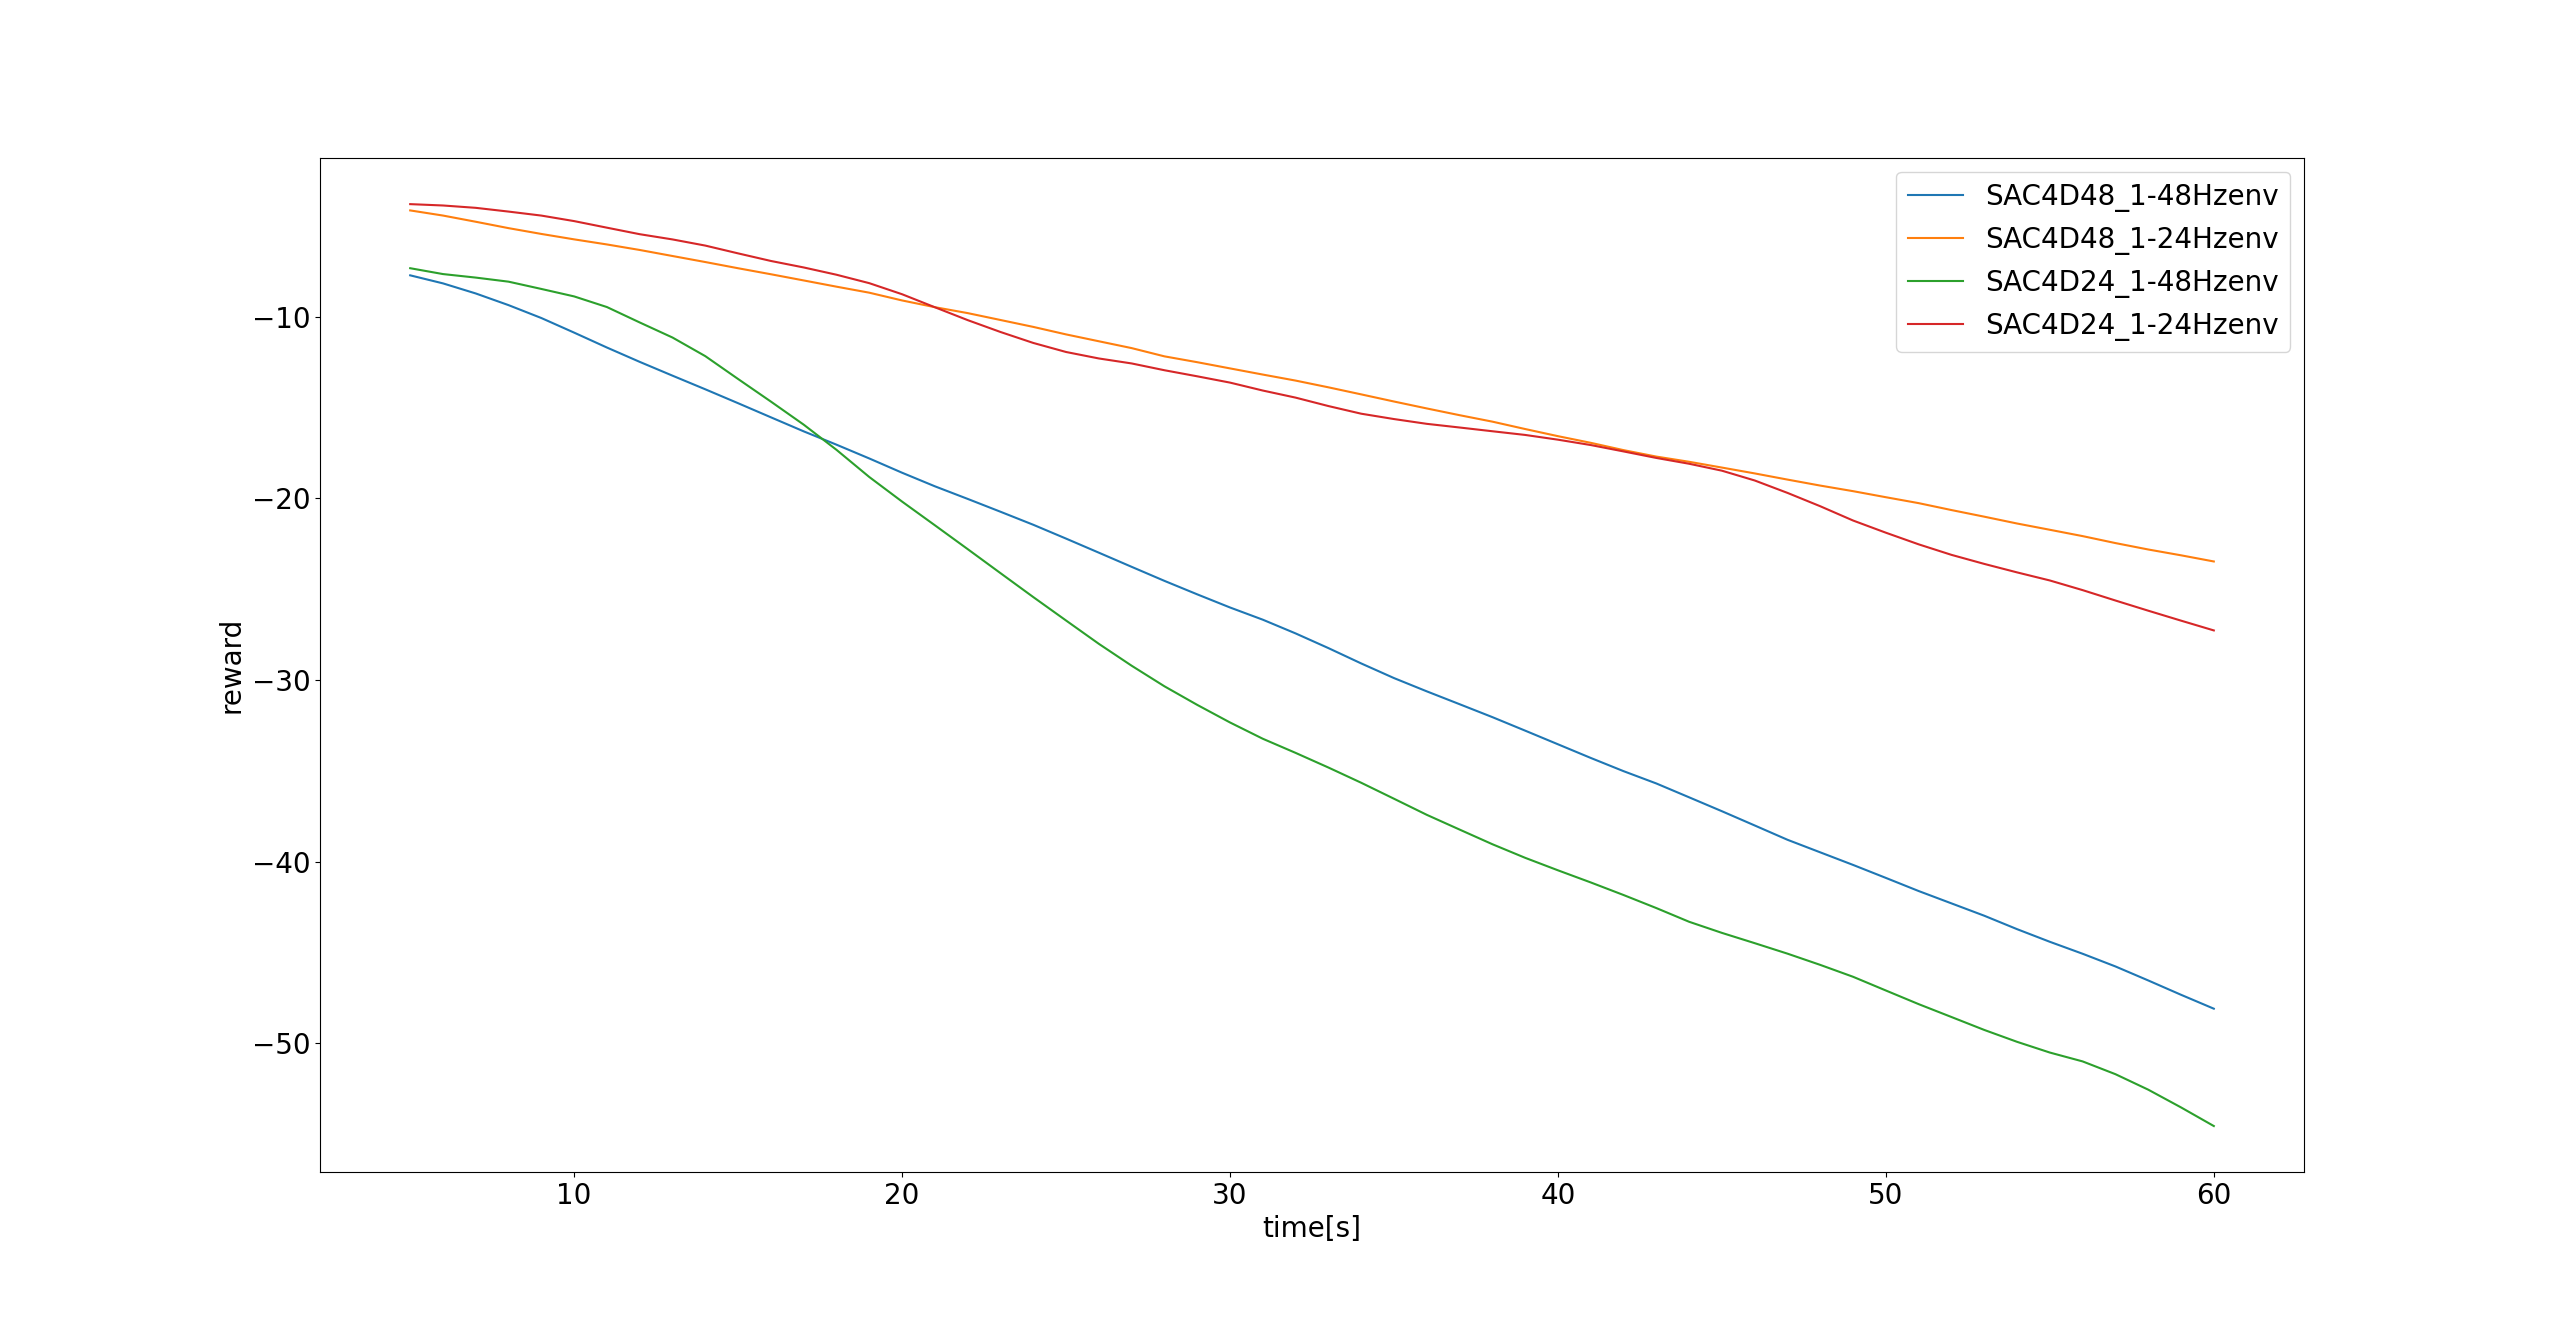
\includegraphics[width=\linewidth]{figures/HzVergleich.png}
	\caption{Performance of SAC4D48\_1 and SAC4D24\_1 on environments with episode lengths between $5s$ and $60s$ and different control frequencies}
	\label{fig:cfv}
\end{figure}



% comparing training
% comparing results (general)
% comparing rpms
% comparing results for different episode lengths



\newpage

\subsection{Random Goal Modes}
On random goal modes the policies are shortly introduced. 
They differ mainly in the type of learning. 
The goal is now sampled with the use of \cref{alg:sample} and not static. 
As a consequence, the complexity of the RL problem increases notably. 
This subsection mainly compares the different training methods and evaluates the resulting models as well as the training per se. 
Also, the models are evaluated for different radii and also radii bigger than the used parsed maximum radius in order to evaluate whether the policies 
can further generalize the problem without the need of learning again with a bigger radius.

\subsubsection{Policies}

\newpage

\begin{longtable}{|c|c|c|c|c|}
	\caption{Overview of the evaluated Policies on random goal modes}\label{tab:pi2}\\
	
	\hline
	Name & Algorithm & ActionType & $\frac{f_s}{\aleph}$ & $t_{total}$ \\
	\hline
	%\toprule
	\endfirsthead
	\caption[]{Overview of the evaluated Policies on fixed goal modes}
	\endhead
	SAC4D\_2.zip & SAC & $rpm$ & $48Hz$ & $1e8$\\
	\hline
	SAC4Dcurri\_2.zip & SAC & $rpm$ & $48Hz$ & $5e7$\\
	\hline
	SAC4Dsp\_curri\_2.zip & SAC & $rpm$ & $48Hz$ & $5e7$\\
	\hline
	$\pi_{opt}$ & & $rpm$ & & \\
	\hline
\end{longtable}
% SAC4D
% SAC4DCurriculum
% SAC4DSelf-PasedCurriculum

% comparing training
% comparing results
% comparing results for different episode lengths and radi
\newpage

\subsubsection{Training Comparison}

\newpage

\subsubsection{Overall Comparison}

\newpage

\subsubsection{Comparison for different radii}
\begin{align}
	\mathbb{E} (dist_0(R)) &= 0.5 + \frac{3}{8} \cdot R \\
	r_{opt}(R) &\approx R \cdot  
\end{align}

\newpage

\subsection{Wind Disruption}

% SAC4D
% SAC4DCurriculum
% SAC4DSelf-PasedCurriculum

% comparing in different wind fields of different strength